


\section{Results}


\begin{frame}[c]{Compared implementations}
    \begin{itemize}[<+(1)->]
        \item 'ICE' - Python implementation
        \item 'KR' - C++ implementation
        \item 'RUST' - this implementation
    \end{itemize}
\end{frame}



\begin{frame}[c,fragile]{Data for Testing}
    \normalsize
    \begin{tabular}{@{}lrr@{}}
        % \textbf{Matrix Details} & & & \\
        \textbf{Name}       & 25kb          & 50kb \\
        \hline
        Filesize            & 1.1 GByte     & 0.73 GByte     \\
        Size                & \verb|123,841|       & \verb|61,928| \\
        Bin length          & \verb|25,000|        & \verb|50,000| \\
        Non-zero elements   & \verb|1,530,533,003| & \verb|1,053,216,825| \\
    \end{tabular}
    % Data from \cite{rao20143d}.
\end{frame}




\begin{frame}[c]{Memory Requirements during correction}
    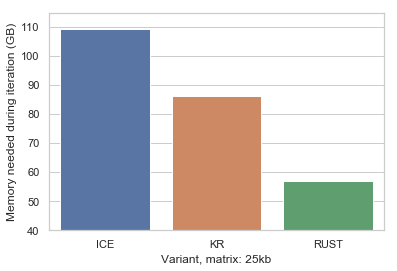
\includegraphics[scale=0.8]{memiter_25}
\end{frame}


\begin{frame}[c]{Peak Memory Usage}
    \only<1>{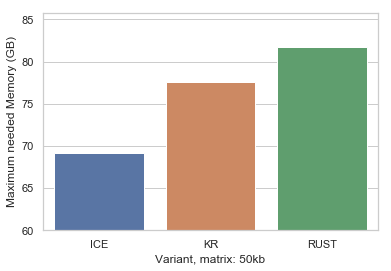
\includegraphics[scale=0.8]{maxresident_50}}
    \only<2>{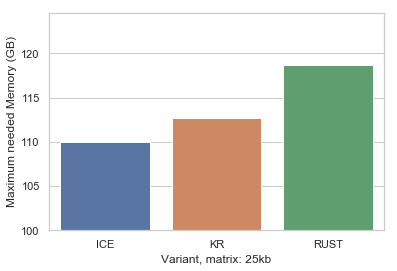
\includegraphics[scale=0.8]{maxresident_25}}
    \only<3>{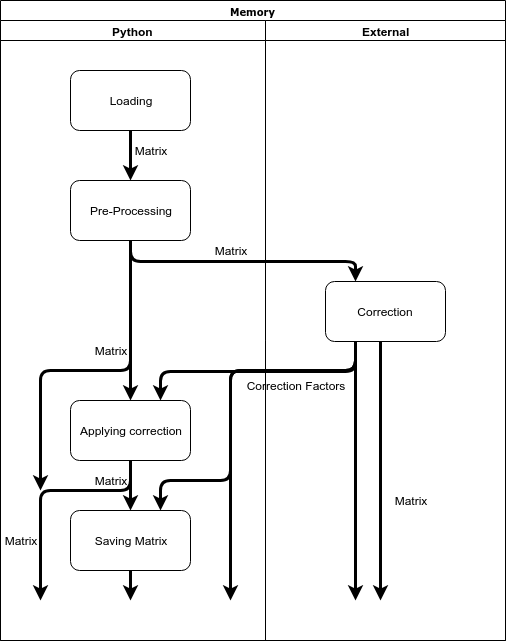
\includegraphics[scale=0.35]{correction_process}}
\end{frame}

\begin{frame}[c]{Comparison of Memory needs}
    \begin{tabular}{lrrr}
        \textbf{Memory needs Comparison} & ICE & KR & RUST \\
        \hline
        During correction (50kb) &   54.6 & 43.1 & \textbf{39.0}   \\
        Maximum          (50kb) &   \textbf{69.2} & 77.6 & 81.7 \\
        During correction (25kb) &   110.0 & 86.0 & \textbf{57.0}  \\
        Maximum          (25kb) &   \textbf{110.0} & 112.7 & 118.6 \\
    \end{tabular}
\end{frame}


% \begin{frame}[c]{Loading Times}
%     \only<2>{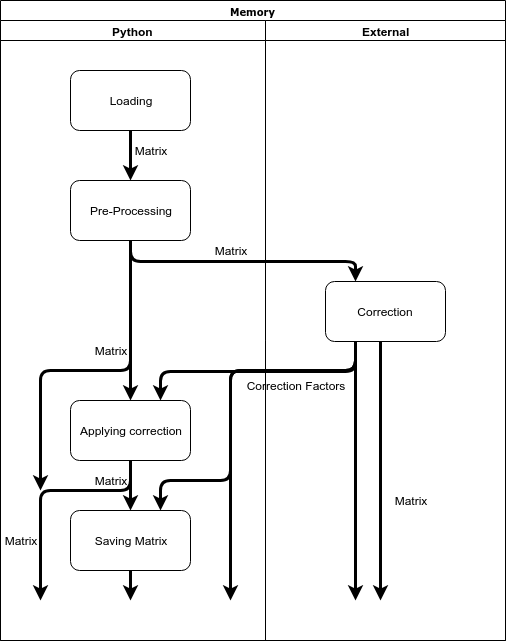
\includegraphics[scale=0.35]{correction_process}}
%     \only<3>{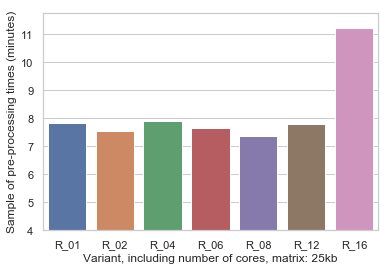
\includegraphics[scale=0.8]{loadtimes_25}}
%     \only<4>{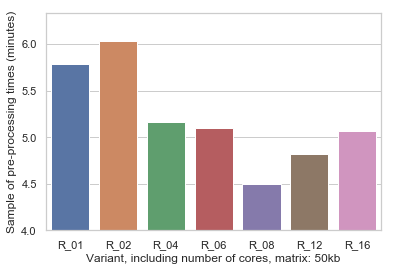
\includegraphics[scale=0.8]{loadtimes_50}}
% \end{frame}


\begin{frame}[c]{Runtime Length}
    \only<2>{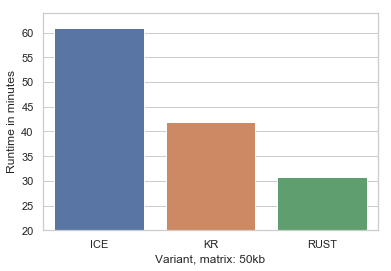
\includegraphics[scale=0.8]{runtime_50}}
    \only<3>{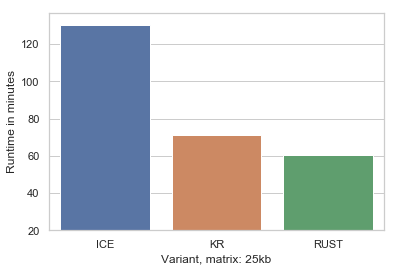
\includegraphics[scale=0.8]{runtime_25}}
\end{frame}


\begin{frame}[c]{Control Flow Diagram}
    \pause
    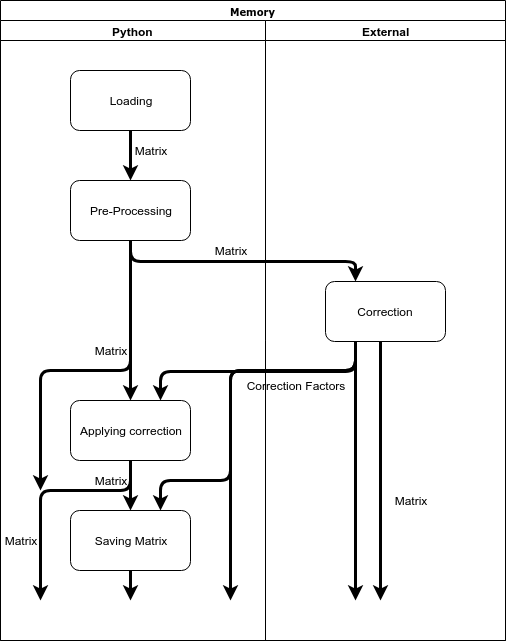
\includegraphics[scale=0.35]{correction_process}
\end{frame}


\begin{frame}[c]{Multicore Runtime Length Comparison}
    % \only<2>{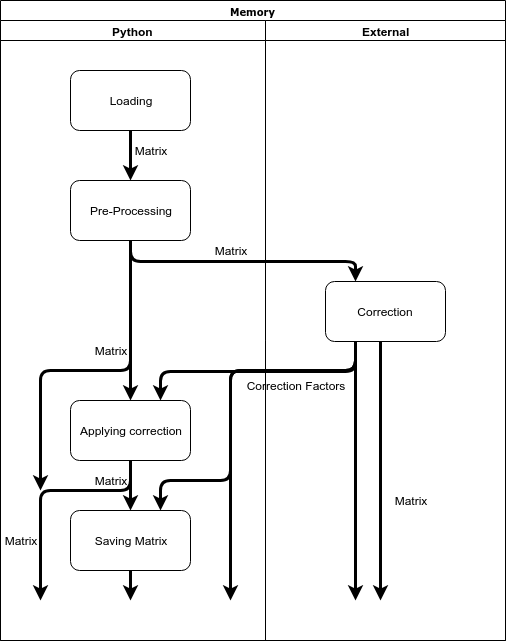
\includegraphics[scale=0.35]{correction_process}}
    \only<2>{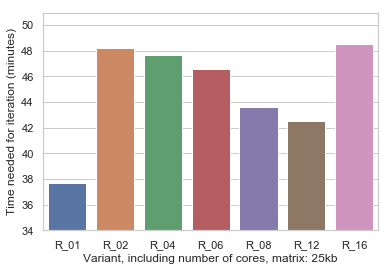
\includegraphics[scale=0.8]{compute_multi_25}}
    \only<3>{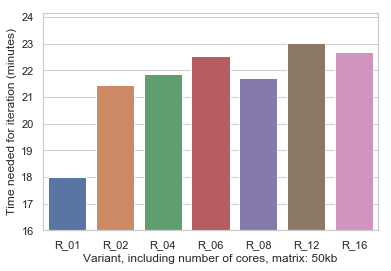
\includegraphics[scale=0.8]{runtime_multi_50}}
\end{frame}

\begin{frame}[c]{Overall Runtime Length Comparison}
    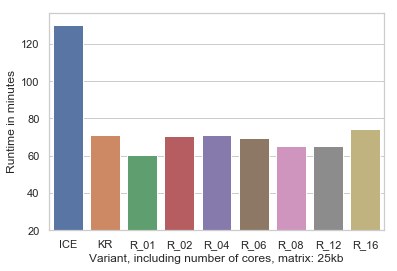
\includegraphics[scale=0.8]{runtime_multi_25}
\end{frame}

\begin{frame}[c]{Multicore Memory Comparison}
    \only<2>{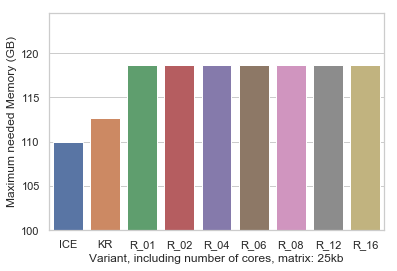
\includegraphics[scale=0.8]{maxresident_multi_25}}
    \only<3>{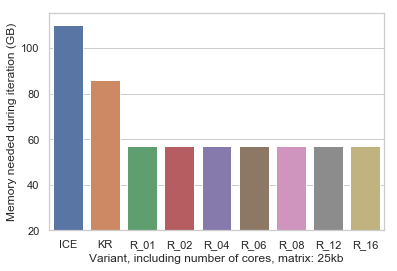
\includegraphics[scale=0.8]{memiter_multi_25}}
\end{frame}



\begin{frame}[c]{Comparison of Results}
    \begin{figure}
    \subfloat[Uncorrected]{
    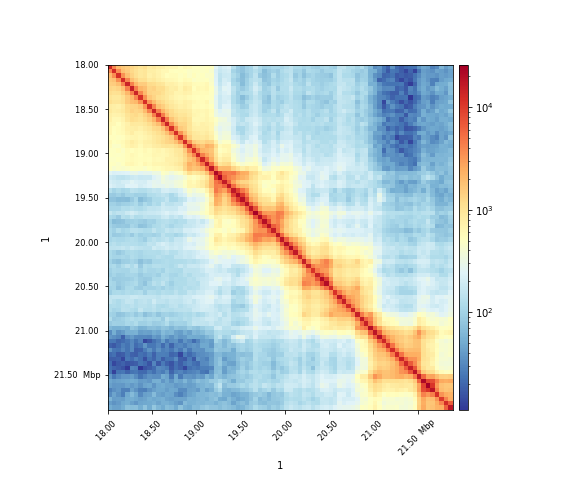
\includegraphics[scale=0.205, trim=50 45 50 30,clip]{c_50kb}}
    \subfloat[RUST]{           
    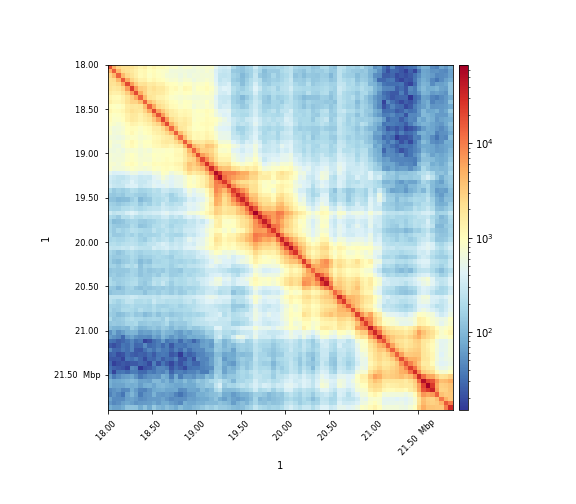
\includegraphics[scale=0.205, trim=50 45 50 30,clip]{c_rust_50kb}} \\
    \subfloat[KR]{             
    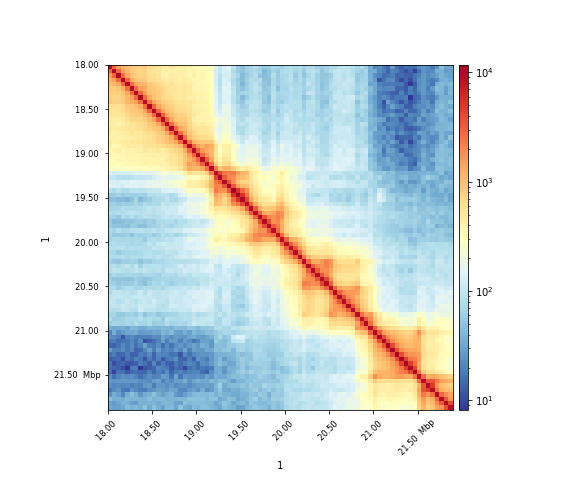
\includegraphics[scale=0.205, trim=50 45 50 30,clip]{c_kr_50kb}}
    \subfloat[ICE]{            
    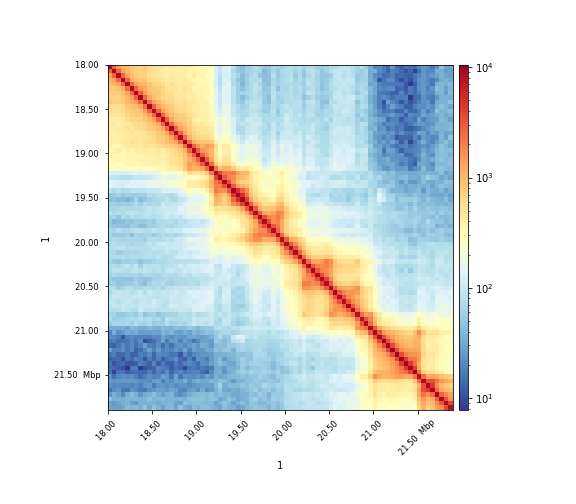
\includegraphics[scale=0.205, trim=50 45 50 30,clip]{c_ice_50kb}}
    \end{figure}
\end{frame}

